\documentclass[tikz, border=15pt]{standalone}
\usepackage{amsmath, amssymb}

\begin{document}
	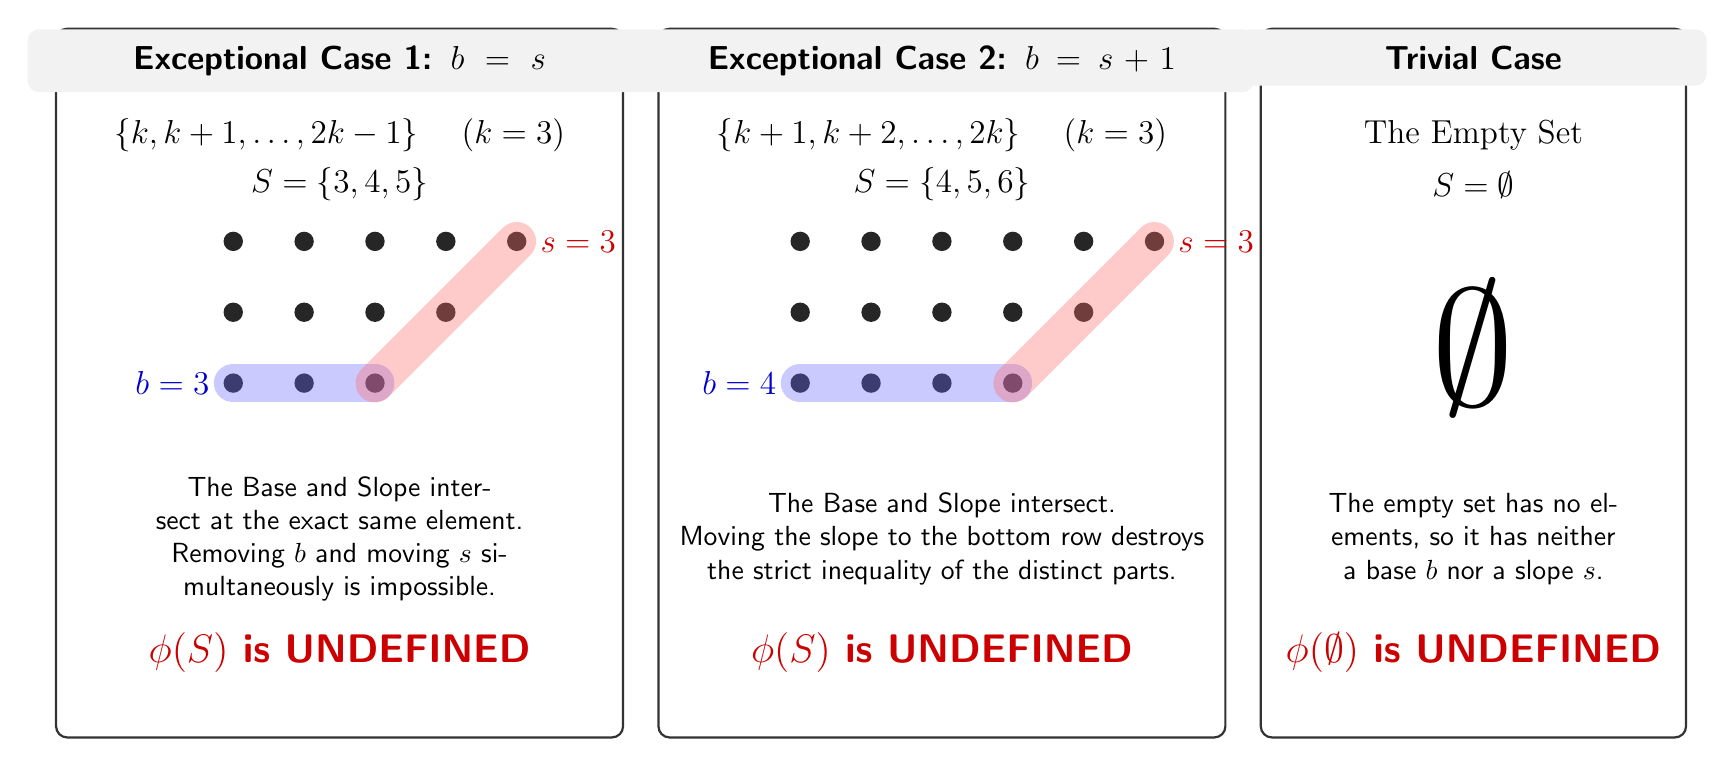
\begin{tikzpicture}[
		scale=0.9,
		dot/.style={circle, fill=black!85, minimum size=7pt, inner sep=0pt},
		base hl/.style={blue!60, line width=14pt, opacity=0.35, line cap=round},
		slope hl/.style={red!60, line width=14pt, opacity=0.35, line cap=round},
		panel frame/.style={draw=black!80, thick, rounded corners=4pt},
		panel title/.style={fill=black!5, text width=7.5cm, align=center, font=\sffamily\large\bfseries, inner sep=6pt, rounded corners=4pt},
		math text/.style={font=\large},
		desc text/.style={font=\sffamily, align=center, text width=7cm}
		]
		
		% =========================================================
		% Panel 1: Case 1 (b = s)
		% =========================================================
		\begin{scope}[xshift=0cm]
			% Panel Background and Title
			\draw[panel frame] (0,0) rectangle (8, 10);
			\node[panel title, anchor=north] at (4, 10) {Exceptional Case 1: $b = s$};
			
			% Subtitle / Set Definition
			\node[math text] at (4, 8.5) {$\{k, k+1, \dots, 2k-1\}$ \quad ($k=3$)};
			\node[math text] at (4, 7.8) {$S = \{3, 4, 5\}$};
			
			% Dot Diagram (Centered roughly around x=4)
			\begin{scope}[xshift=1.5cm, yshift=4cm]
				\foreach \y/\n in {3/5, 2/4, 1/3} {
					\foreach \x in {1,...,\n} {
						\node[dot] at (\x, \y) {};
					}
				}
				% Highlights
				\draw[base hl] (1,1) -- (3,1);
				\draw[slope hl] (5,3) -- (3,1);
				
				% Labels
				\node[blue!80!black, left, font=\large] at (0.8, 1) {$b=3$};
				\node[red!80!black, right, font=\large] at (5.2, 3) {$s=3$};
			\end{scope}
			
			% Intersection Note
			\node[desc text] at (4, 2.8) {The Base and Slope intersect at the exact same element.\\Removing $b$ and moving $s$ simultaneously is impossible.};
			
			% Undefined symbol
			\node[font=\sffamily\Large\bfseries, red!80!black] at (4, 1.2) {$\phi(S)$ is UNDEFINED};
		\end{scope}
		
		% =========================================================
		% Panel 2: Case 2 (b = s + 1)
		% =========================================================
		\begin{scope}[xshift=8.5cm]
			% Panel Background and Title
			\draw[panel frame] (0,0) rectangle (8, 10);
			\node[panel title, anchor=north] at (4, 10) {Exceptional Case 2: $b = s + 1$};
			
			% Subtitle / Set Definition
			\node[math text] at (4, 8.5) {$\{k+1, k+2, \dots, 2k\}$ \quad ($k=3$)};
			\node[math text] at (4, 7.8) {$S = \{4, 5, 6\}$};
			
			% Dot Diagram (Centered roughly around x=4)
			\begin{scope}[xshift=1cm, yshift=4cm]
				\foreach \y/\n in {3/6, 2/5, 1/4} {
					\foreach \x in {1,...,\n} {
						\node[dot] at (\x, \y) {};
					}
				}
				% Highlights
				\draw[base hl] (1,1) -- (4,1);
				\draw[slope hl] (6,3) -- (4,1);
				
				% Labels
				\node[blue!80!black, left, font=\large] at (0.8, 1) {$b=4$};
				\node[red!80!black, right, font=\large] at (6.2, 3) {$s=3$};
			\end{scope}
			
			% Intersection Note
			\node[desc text] at (4, 2.8) {The Base and Slope intersect.\\Moving the slope to the bottom row destroys the strict inequality of the distinct parts.};
			
			% Undefined symbol
			\node[font=\sffamily\Large\bfseries, red!80!black] at (4, 1.2) {$\phi(S)$ is UNDEFINED};
		\end{scope}
		
		% =========================================================
		% Panel 3: The Empty Set
		% =========================================================
		\begin{scope}[xshift=17cm]
			% Panel Background and Title
			\draw[panel frame] (0,0) rectangle (6, 10);
			\node[panel title, anchor=north, text width=5.5cm] at (3, 10) {Trivial Case};
			
			% Subtitle / Set Definition
			\node[math text] at (3, 8.5) {The Empty Set};
			\node[math text] at (3, 7.8) {$S = \emptyset$};
			
			% Huge Empty Set Symbol
			\node[scale=6] at (3, 5.5) {$\emptyset$};
			
			% Note
			\node[desc text, text width=5cm] at (3, 2.8) {The empty set has no elements, so it has neither a base $b$ nor a slope $s$.};
			
			% Undefined symbol
			\node[font=\sffamily\Large\bfseries, red!80!black] at (3, 1.2) {$\phi(\emptyset)$ is UNDEFINED};
		\end{scope}
		
	\end{tikzpicture}
\end{document}

%\documentclass[tikz, border=20pt]{standalone}
%\usepackage{amsmath, amssymb}
%
%\begin{document}
%	\begin{tikzpicture}[
%		scale=0.75,
%		dot/.style={circle, fill=black, minimum size=7pt, inner sep=0pt},
%		base highlight/.style={blue!70!black, line width=12pt, opacity=0.3, line cap=round},
%		slope highlight/.style={red!70!black, line width=12pt, opacity=0.3, line cap=round},
%		label blue/.style={text=blue!90!black, font=\sffamily\bfseries},
%		label red/.style={text=red!90!black, font=\sffamily\bfseries},
%		main title/.style={font=\sffamily\bfseries\LARGE},
%		panel title/.style={font=\sffamily\bfseries\large, align=center},
%		arrow label/.style={font=\sffamily\small, align=center},
%		annotation/.style={font=\sffamily\small, align=center}
%		]
%		
%		% =========================================================
%		% Main Title
%		% =========================================================
%		\node[main title] at (22, 6.5) {Franklin's Map $\phi$: Complete Exceptional Cases (Fixed Points)};
%		
%		
%		% =========================================================
%		% Panel 1: Standard Mapping Case (Non-Exceptional)
%		% =========================================================
%		\begin{scope}[xshift=0cm]
%			% Panel Title
%			\node[panel title, anchor=north] at (1, 5) {Standard Mapping Case\\[2pt](Non-Exceptional)};
%			
%			% S = {2, 4, 5, 6} sub-diagram
%			\begin{scope}[yshift=0.5cm]
%				\foreach \y/\n in {1/2, 2/4, 3/5, 4/6} {
%					\foreach \x in {0,...,\numexpr\n-1\relax} {
%						\node[dot] at (\x, \y) {};
%					}
%				}
%				% Highlights
%				\draw[base highlight] (0,1) -- (1,1);
%				\draw[slope highlight] (5,4) -- (4,3) -- (3,2);
%				
%				% Labels
%				\node[label blue, anchor=north] at (1, 1) {b=2};
%				\node[label red, anchor=south west] at (5, 4) {s=3};
%				
%				% Text Below
%%				\node[annotation, text width=4cm] at (current scope.south) {S = \{2, 4, 5, 6\}\\[4pt] Map $\phi$ is defined};
%			\end{scope}
%			
%			% Mapping Arrow
%			\draw[->, ultra thick, >=stealth] (7.5, 3) -- (9.5, 3);
%			
%			% phi(S) = {4, 6, 7} sub-diagram
%			\begin{scope}[xshift=10cm, yshift=0.5cm]
%				\foreach \y/\n in {1/4, 2/6, 3/7} {
%					\foreach \x in {0,...,\numexpr\n-1\relax} {
%						\node[dot] at (\x, \y) {};
%					}
%				}
%				
%				% Text Below
%%				\node[annotation, text width=4cm] at (current scope.south) {\(\phi(S) = \{4, 6, 7\}\)};
%			\end{scope}
%		\end{scope}
%		
%		
%		% =========================================================
%		% Panel 2: Exceptional Fixed Point 1: b=s
%		% =========================================================
%		\begin{scope}[xshift=22cm]
%			% Panel Title
%			\node[panel title, anchor=north] at (1, 5) {Exceptional Fixed\\[2pt]Point 1: $b=s$};
%			
%			% S = {3, 4, 5} diagram for k=3
%			\begin{scope}[yshift=0.5cm]
%				\foreach \y/\n in {1/3, 2/4, 3/5} {
%					\foreach \x in {0,...,\numexpr\n-1\relax} {
%						\node[dot] at (\x, \y) {};
%					}
%				}
%				% Highlights
%				\draw[base highlight] (0,1) -- (2,1);
%				\draw[slope highlight] (4,3) -- (3,2) -- (2,1);
%				
%				% Labels
%				\node[label blue, anchor=north] at (1.5, 1) {b=3};
%				\node[label red, anchor=south west] at (4, 3) {s=3};
%				\node[label red, anchor=south east] at (4, 3) {s=3}; % Original redundancy. Let's make it single.
%				
%				% Text Below
%%				\node[annotation, text width=6cm] at (current scope.south) {Case: \(\{k, k+1, \dots, 2k-1\}\) for \(k=3\)};
%			\end{scope}
%			
%			% Mapping Arrow with X
%			\draw[->, ultra thick, >=stealth] (5.5, 3) -- (7.5, 3);
%			\draw[ultra thick, red!90!black] (6.5-0.3, 3-0.3) -- (6.5+0.3, 3+0.3);
%			\draw[ultra thick, red!90!black] (6.5-0.3, 3+0.3) -- (6.5+0.3, 3-0.3);
%			
%			% Arrow Label
%			\node[arrow label, below, yshift=-4pt] at (6.5, 3) {Mapping\\[-2pt]Undefined};
%		\end{scope}
%		
%		
%		% =========================================================
%		% Panel 3: Exceptional Fixed Point 2: b=s+1
%		% =========================================================
%		\begin{scope}[xshift=32cm]
%			% Panel Title
%			\node[panel title, anchor=north] at (1, 5) {Exceptional Fixed\\[2pt]Point 2: $b=s+1$};
%			
%			% S = {4, 5, 6} diagram for k=3
%			\begin{scope}[yshift=0.5cm]
%				\foreach \y/\n in {1/4, 2/5, 3/6} {
%					\foreach \x in {0,...,\numexpr\n-1\relax} {
%						\node[dot] at (\x, \y) {};
%					}
%				}
%				% Highlights
%				\draw[base highlight] (0,1) -- (3,1);
%				\draw[slope highlight] (5,3) -- (4,2) -- (3,1);
%				
%				% Labels
%				\node[label blue, anchor=north] at (1.5, 1) {b=4};
%				\node[label red, anchor=south west] at (5, 3) {s=3};
%				
%				% Text Below
%%				\node[annotation, text width=6cm] at (current scope.south) {Case: \(\{k+1, k+2, \dots, 2k\}\) for \(k=3\)};
%			\end{scope}
%			
%			% Mapping Arrow with X
%			\draw[->, ultra thick, >=stealth] (7.5, 3) -- (9.5, 3);
%			\draw[ultra thick, red!90!black] (8.5-0.3, 3-0.3) -- (8.5+0.3, 3+0.3);
%			\draw[ultra thick, red!90!black] (8.5-0.3, 3+0.3) -- (8.5+0.3, 3-0.3);
%			
%			% Arrow Label
%			\node[arrow label, below, yshift=-4pt] at (8.5, 3) {Mapping\\[-2pt]Undefined};
%		\end{scope}
%		
%		
%		% =========================================================
%		% Bottom Note
%		% =========================================================
%		\node[annotation, font=\sffamily\small] at (22, -1.5) {Note: The empty set \(\emptyset\) is also a trivial exception, as it has no base or slope.};
%		
%		
%	\end{tikzpicture}
%\end{document}


%\documentclass[tikz, border=20pt]{standalone}
%\usepackage{amsmath, amssymb}
%\usetikzlibrary{decorations.pathreplacing, calc}
%
%\begin{document}
%	\begin{tikzpicture}[
%		scale=0.8,
%		dot/.style={circle, fill=black!85, minimum size=6pt, inner sep=0pt},
%		movedot/.style={circle, fill=red, minimum size=6pt, inner sep=0pt},
%		movearrow/.style={dashed, red, thick, ->, >=stealth, bend left=25},
%		highlight base/.style={blue!70, line width=16pt, opacity=0.25, line cap=round},
%		highlight slope/.style={red!70, line width=16pt, opacity=0.25, line cap=round}
%		]
%		
%		% =========================================================
%		% CASE 1: b <= s (Move Base to Slope)
%		% Example: S = {2, 4, 5, 6}. b = 2, s = 3. b <= s.
%		% =========================================================
%		\node[anchor=west, font=\sffamily\LARGE\bfseries] at (-0.5, 10.5) {Case 1: $b \le s$ (Move Base)};
%		
%		% --- Left Side: S ---
%		\begin{scope}[xshift=0cm, yshift=4cm]
%			\node[anchor=west, font=\sffamily\Large] at (0, 6) {Partition $S = \{a_1 < a_2 < a_3 < a_4\} = \{2, 4, 5, 6\}$};
%			\node[anchor=west, font=\sffamily] at (0.2, 5.2) {Base $b=2$ (blue), Slope $s=3$ (red)};
%			
%			% Draw static dots
%			\foreach \y/\n in {4/6, 3/5, 2/4} {
%				\foreach \x in {1,...,\n} {
%					\node[dot] at (\x, \y) {};
%				}
%			}
%			% Draw moved dots (the base)
%			\node[movedot] (b1) at (1, 1) {};
%			\node[movedot] (b2) at (2, 1) {};
%			
%			% Highlights
%			\draw[highlight base] (1, 1) -- (2, 1);
%			\draw[highlight slope] (6, 4) -- (4, 2);
%			
%			% Weight Annotation
%			\node[anchor=north west, font=\sffamily, align=left] at (0, -0.2) {
%				$\sum_{j \in S} j = 6+5+4+2 = \mathbf{17}$\\[4pt]
%				$\#S = 4$ (Even)\\[4pt]
%				Weight: $(-1)^{\#S} q^{\sum j} = \mathbf{+q^{17}}$
%			};
%		\end{scope}
%		
%		% --- Mapping Arrow (phi) ---
%		\draw[->, ultra thick, >=stealth] (7.5, 6.5) -- (10.5, 6.5) node[midway, above, font=\Large] {$\phi(S)$};
%		% Curved arrows showing dot movement
%		\draw[movearrow] (2.2, 5) -- (7.5, 8); % b2 to new s position 2
%		\draw[movearrow] (1.2, 5) -- (6.5, 7); % b1 to new s position 1
%		
%		% --- Right Side: \phi(S) ---
%		\begin{scope}[xshift=12cm, yshift=4cm]
%			\node[anchor=west, font=\sffamily\Large] at (0, 6) {Result $\phi(S) = \{4, 6, 7\}$};
%			\node[anchor=west, font=\sffamily] at (0.2, 5.2) {Base $b=4$, Slope $s=2$. $b > s \to$ Case 2 next.};
%			
%			% Draw static dots (same as left, y=1 row removed)
%			\foreach \y/\n in {4/6, 3/5, 2/4} {
%				\foreach \x in {1,...,\n} {
%					\node[dot] at (\x, \y) {};
%				}
%			}
%			% Draw newly arrived dots (added to the slope)
%			\node[movedot] (s1) at (7, 4) {};
%			\node[movedot] (s2) at (6, 3) {};
%			
%			% Highlights
%			\draw[highlight base] (1, 2) -- (4, 2);
%			\draw[highlight slope] (7, 4) -- (6, 3);
%			
%			% Weight Annotation
%			\node[anchor=north west, font=\sffamily, align=left] at (0, -0.2) {
%				$\sum_{j \in \phi(S)} j = 7+6+4 = \mathbf{17}$\\[4pt]
%				$\#\phi(S) = 3$ (Odd)\\[4pt]
%				Weight: $(-1)^{\#\phi(S)} q^{\sum j} = \mathbf{-q^{17}}$
%			};
%		\end{scope}
%		
%		
%		% =========================================================
%		% CASE 2: b > s (Move Slope to Base)
%		% Example: S' = {4, 6, 7}. b = 4, s = 2. b > s.
%		% =========================================================
%		\node[anchor=west, font=\sffamily\LARGE\bfseries] at (-0.5, -1.5) {Case 2: $b > s$ (Move Slope)};
%		
%		% --- Left Side: S' ---
%		\begin{scope}[xshift=0cm, yshift=-8cm]
%			\node[anchor=west, font=\sffamily\Large] at (0, 6) {Partition $S' = \{a_1 < a_2 < a_3\} = \{4, 6, 7\}$};
%			\node[anchor=west, font=\sffamily] at (0.2, 5.2) {Base $b=4$ (blue), Slope $s=2$ (red)};
%			
%			% Draw static dots
%			\foreach \y/\n in {4/6, 3/5, 2/4} {
%				\foreach \x in {1,...,\n} {
%					\node[dot] at (\x, \y) {};
%				}
%			}
%			% Draw moved dots (the slope)
%			\node[movedot] (sm1) at (7, 4) {};
%			\node[movedot] (sm2) at (6, 3) {};
%			
%			% Highlights
%			\draw[highlight base] (1, 2) -- (4, 2);
%			\draw[highlight slope] (7, 4) -- (6, 3);
%			
%			% Weight Annotation
%			\node[anchor=north west, font=\sffamily, align=left] at (0, -0.2) {
%				Sum = $\mathbf{17}$\\[4pt]
%				Elements = $3$ (Odd)\\[4pt]
%				Weight: $\mathbf{-q^{17}}$
%			};
%		\end{scope}
%		
%		% --- Mapping Arrow (phi inverse) ---
%		\draw[->, ultra thick, >=stealth] (7.5, -5.5) -- (10.5, -5.5) node[midway, above, font=\Large] {$\phi^{-1}(S') = \phi(S')$};
%		% Curved arrows showing dot movement
%		\draw[movearrow] (7.2, -4) -- (2.5, -7); % sm1 to new b position 2
%		\draw[movearrow] (6.2, -5) -- (1.5, -7); % sm2 to new b position 1
%		
%		% --- Right Side: S'' (Inverse mapped result) ---
%		\begin{scope}[xshift=12cm, yshift=-8cm]
%			\node[anchor=west, font=\sffamily\Large] at (0, 6) {Result $\phi(S') = \{2, 4, 5, 6\}$};
%			\node[anchor=west, font=\sffamily] at (0.2, 5.2) {Back at S from Case 1 ($b \le s$). Map is an involution.};
%			
%			% Draw static dots (same as above)
%			\foreach \y/\n in {4/6, 3/5, 2/4} {
%				\foreach \x in {1,...,\n} {
%					\node[dot] at (\x, \y) {};
%				}
%			}
%			% Draw newly arrived dots (forming the new base element s)
%			\node[movedot] (b1_end) at (1, 1) {};
%			\node[movedot] (b2_end) at (2, 1) {};
%			
%			% Highlights
%			\draw[highlight base] (1, 1) -- (2, 1);
%			\draw[highlight slope] (6, 4) -- (4, 2);
%			
%			% Weight Annotation
%			\node[anchor=north west, font=\sffamily, align=left] at (0, -0.2) {
%				Sum = $\mathbf{17}$\\[4pt]
%				Elements = $4$ (Even)\\[4pt]
%				Weight: $\mathbf{+q^{17}}$
%			};
%		\end{scope}
%		
%	\end{tikzpicture}
%\end{document}


%\documentclass[tikz, border=20pt]{standalone}
%\usepackage{amsmath, amssymb}
%\usetikzlibrary{decorations.pathreplacing}
%
%\begin{document}
%	\begin{tikzpicture}[
%		scale=0.9,
%		dot/.style={circle, fill=black!85, minimum size=6.5pt, inner sep=0pt},
%		highlight base/.style={blue!70, line width=16pt, opacity=0.3, line cap=round},
%		highlight slope/.style={red!70, line width=16pt, opacity=0.3, line cap=round}
%		]
%		
%		% ---------------------------------------------------------
%		% Row 7: a_r (Top element)
%		% ---------------------------------------------------------
%		\node[left, font=\large] at (0, 7) {$a_r$};
%		\node[dot] at (1, 7) {}; 
%		\node[dot] at (2, 7) {}; 
%		\node at (5.5, 7) {$\cdots$}; 
%		\node[dot] at (10, 7) {};
%		
%		% ---------------------------------------------------------
%		% Row 6: a_{r-1} (Second element)
%		% ---------------------------------------------------------
%		\node[left, font=\large] at (0, 6) {$a_{r-1}$};
%		\node[dot] at (1, 6) {}; 
%		\node[dot] at (2, 6) {}; 
%		\node at (5, 6) {$\cdots$}; 
%		\node[dot] at (9, 6) {};
%		
%		% ---------------------------------------------------------
%		% Row 5: Vertical gap within the slope block
%		% ---------------------------------------------------------
%		\node[left, font=\large] at (0, 5) {$\vdots$};
%		\node at (1, 5) {$\vdots$}; 
%		\node at (2, 5) {$\vdots$}; 
%		\node at (8, 5) {$\ddots$}; % Diagonal continuation of slope
%		
%		% ---------------------------------------------------------
%		% Row 4: a_{r-s+1} (Bottom of the slope block)
%		% ---------------------------------------------------------
%		\node[left, font=\large] at (0, 4) {$a_{r-s+1}$};
%		\node[dot] at (1, 4) {}; 
%		\node[dot] at (2, 4) {}; 
%		\node at (4, 4) {$\cdots$}; 
%		\node[dot] at (7, 4) {};
%		
%		% ---------------------------------------------------------
%		% Row 2.5: Vertical gap for the rest of the set S
%		% (Elements are strictly decreasing, but not necessarily consecutive)
%		% ---------------------------------------------------------
%		\node[left, font=\large] at (0, 2.5) {$\vdots$};
%		\node at (1, 2.5) {$\vdots$}; 
%		\node at (2, 2.5) {$\vdots$}; 
%		\node at (5.5, 2.5) {$\ddots$}; 
%		
%		% ---------------------------------------------------------
%		% Row 1: a_1 (Base element)
%		% ---------------------------------------------------------
%		\node[left, font=\large] at (0, 1) {$a_1$};
%		\node[dot] at (1, 1) {}; 
%		\node[dot] at (2, 1) {}; 
%		\node at (2.5, 1) {$\cdots$}; 
%		\node[dot] at (4, 1) {};
%		
%		
%		% =========================================================
%		% Highlights and Annotations
%		% =========================================================
%		
%		% Highlight Base
%		\draw[highlight base] (1,1) -- (4,1);
%		
%		% Brace for Base
%		\draw[decorate, decoration={brace, amplitude=8pt, mirror}, thick, blue!80!black] 
%		(1, 0.5) -- (4, 0.5) 
%		node[midway, below=10pt, font=\large] {Base $b := a_1$};
%		
%		% Highlight Slope (From top-right to bottom-left of the consecutive block)
%		\draw[highlight slope] (10,7) -- (7,4);
%		
%		% Brace for Slope
%		\draw[decorate, decoration={brace, amplitude=10pt}, thick, red!80!black] 
%		(10.3, 7.3) -- (7.3, 4.3) 
%		node[midway, above right=12pt, align=left, font=\large] {Slope $s$};
%		
%		% Text defining the slope property
%		\node[anchor=west, red!80!black, align=left] at (10.5, 5.8) {
%			Consecutive block:\\[4pt]
%			$a_r = a_{r-1}+1 = \dots = a_{r-s+1} + (s-1)$
%		};
%		
%	\end{tikzpicture}
%\end{document}